%===========================================================================
% CHAPITRE 3 — Implémentation et Réalisations
% Mémoire CHOUFA Zouhair — Master BIBDA
% Université Chouaib Doukkali — Faculté des Sciences El Jadida
% Encadrant : Pr. A. Madani
%===========================================================================
\chapter{Implémentation et Réalisations}
\label{chap:implementation}
%===========================================================================

%-----------------------------------------------------------------------
\section{Introduction et Objectifs du Chapitre}
\label{sec:chap3_intro}
%-----------------------------------------------------------------------

Les chapitres précédents ont positionné notre contribution dans l'espace
des travaux existants (Chapitre~\ref{chap:etat_art}) et en ont décrit
l'architecture théorique (Chapitre~\ref{chap:methodologie}). Le présent
chapitre constitue la phase de \textbf{validation concrète}~: il s'agit
de décrire, composant par composant, les décisions d'implémentation
effectives qui ont permis de faire fonctionner le pipeline de
transformation de données tabulaires hétérogènes en Knowledge Graph,
dans un environnement Cloud réel.

Ce chapitre s'articule autour de cinq modules séquentiels et
interdépendants, numérotés de 0 à 4. Le \textbf{Module~0} constitue une
étape préalable indispensable~: la génération contrôlée des données de
vérité terrain (\textit{Ground Truth}), sans laquelle aucune évaluation
rigoureuse du pipeline ne serait possible. Le \textbf{Module~1}
réalise l'ingestion des sources brutes et leur profilage qualité
automatique. Le \textbf{Module~2} met en œuvre le cœur scientifique de
la contribution~: le schema matching hybride combinant embeddings
Sentence-BERT et agent LLM à faible coût. Le \textbf{Module~3}
opère la triplification sémantique déclarative via le moteur
Morph-KGC et des règles YARRRML auto-générées. Enfin, le
\textbf{Module~4} réconcilie les entités issues des deux sources grâce
au modèle probabiliste de Splink et génère les ponts sémantiques
\texttt{owl:sameAs} constituant le graphe unifié final.

La section~\ref{sec:env_travail} présente l'environnement de travail
et l'orchestration générale. Les sections~\ref{sec:module0}
à~\ref{sec:module4} détaillent chaque module successivement. Afin de
ne pas se limiter à une description purement fonctionnelle des
résultats, la section~\ref{sec:ablation_module2} présente une
\textbf{étude d'ablation comparative} isolant la contribution propre
de chacun des deux composants du Module~2 (SBERT et agent LLM) par
rapport à l'architecture hybride complète. La
section~\ref{sec:deploiement} décrit le déploiement dans le triplestore
et la visualisation du graphe produit.
%-----------------------------------------------------------------------
\section{Environnement de Travail et Outils}
\label{sec:env_travail}
%-----------------------------------------------------------------------

\subsection{Plateforme Cloud~: Lightning.ai}
\label{subsec:lightning}

L'intégralité du pipeline a été développée et exécutée sur la plateforme
Cloud \textbf{Lightning.ai}~\cite{lightningai2024}. Ce choix architectural
répond à une contrainte pratique identifiée dès la phase de conception~:
la combinaison de modèles d'embeddings à inférence locale
(Sentence-BERT), de comparaisons probabilistes sur des matrices de grande
taille (Splink/DuckDB), et de génération de triplets RDF à la volée
(Morph-KGC) impose des ressources de calcul dépassant les capacités d'un
poste local standard. Lightning.ai offre un environnement isolé,
reproductible et accessible via navigateur, dans lequel chaque session
dispose d'un conteneur dédié avec système de fichiers persistant et
connexion Internet vers les APIs externes --- notamment l'API Groq
utilisée pour l'inférence LLM.

Cette isolation garantit la reproductibilité des expériences~: à partir
du dépôt Git du projet et des fichiers sources, un tiers peut reproduire
exactement l'environnement d'exécution et obtenir des résultats
identiques, sans configuration manuelle de dépendances systèmes. Le
langage de programmation retenu est \textbf{Python~3.10}, dont la
maturité de l'écosystème scientifique (\texttt{pandas}, \texttt{rdflib},
\texttt{sentence-transformers}) et la compatibilité avec l'ensemble des
bibliothèques sélectionnées en font le choix naturel pour ce type de
pipeline de traitement de données sémantiques.

\subsection{Orchestration~: le script maître \texttt{run\_pipeline.py}}
\label{subsec:orchestration}

L'ensemble des modules a été orchestré par un script maître unique,
\texttt{run\_pipeline.py}, exposant une interface en ligne de commande
(CLI) construite avec le module standard \texttt{argparse}. Ce script
accepte deux drapeaux principaux~:

\begin{itemize}
    \item \texttt{from MODULE\_N}~: reprend l'exécution à partir du
    module numéroté $N$, en réutilisant les artefacts intermédiaires
    déjà produits par les modules précédents. Ce mécanisme est essentiel
    en phase de développement itératif~: il évite de relancer des étapes
    coûteuses (appels API Groq, triplification complète) lors d'un
    ajustement localisé.
  \item \texttt{only MODULE\_N}~: exécute exclusivement le module
    $N$, ce qui permet de valider ou de déboguer un composant en
    isolation sans perturber le reste de la chaîne.
\end{itemize}

\noindent Cette conception est alignée avec le principe de modularité
défendu au Chapitre~\ref{chap:methodologie}~: chaque module produit un
artefact intermédiaire formellement défini, constituant l'interface
contractuelle entre les étapes successives.

\subsection{Journalisation~: \texttt{RotatingFileHandler}}
\label{subsec:logging}

Un système de journalisation centralisé a été mis en place via la
classe \\ \texttt{RotatingFileHandler} du module standard Python
\texttt{logging}. Cette approche est particulièrement pertinente dans
un contexte Big Data, où le volume des traces d'exécution peut
rapidement saturer le système de fichiers disponible. Le handler est
configuré avec une taille maximale de fichier de 5~Mo et une rotation
sur 3 fichiers au maximum, garantissant que les journaux les plus
récents sont toujours accessibles sans risque de saturation du
stockage de la plateforme Lightning.ai.

Chaque entrée de journal inclut l'horodatage précis, le nom du module
émetteur, le niveau de sévérité (\texttt{DEBUG}, \texttt{INFO},
\texttt{WARNING}, \texttt{ERROR}) et le message associé. Cette
granularité facilite le diagnostic post-mortem en cas d'erreur dans
l'un des modules, et constitue une bonne pratique d'ingénierie en
environnement de production. Le tableau~\ref{tab:stack_outils} récapitule
l'ensemble des composants technologiques du pipeline et leurs rôles
respectifs.

\begin{table}[h]
\centering
\caption{Stack technologique consolidée du pipeline --- versions et
         rôles fonctionnels.}
\label{tab:stack_outils}
\begin{tabular}{p{4.8cm}p{1.8cm}p{6cm}}
\hline
\textbf{Composant} & \textbf{Version} & \textbf{Rôle dans le pipeline} \\
\hline
Python                                     & 3.10   & Langage d'orchestration général \\
pandas~\cite{pandas2020}                   & 2.x    & Ingestion et manipulation tabulaire \\
ydata-profiling~\cite{ydataprofiling2023}  & 4.x    & Profilage automatique des sources \\
Faker~\cite{faker2024}                     & 24.x   & Data augmentation (Module~0) \\
sentence-transformers~\cite{reimers2019sbert} & 2.x & Embeddings SBERT (Module~2) \\
LangChain~\cite{langchain2023}        & 0.1.x  & Orchestration de l'agent LLM \\
LLaMA~3.1 via Groq API~\cite{groq2024}    & 8B     & LLM pour cas ambigus (Module~2) \\
tenacity                                   & 8.x    & Résilience des appels API (retry) \\
Morph-KGC~\cite{arenas2023morphkgc}        & 2.x    & Moteur de triplification RML \\
Splink~\cite{splink2023}            & 3.x    & Résolution d'entités probabiliste \\
DuckDB~\cite{raasveldt2019duckdb}                   & 0.10.x & Backend analytique de Splink \\
Ontotext GraphDB~\cite{ontotext2024graphdb}        & 10.x   & Triple store SPARQL (Module~5) \\
PyVis~\cite{pyvis2023}                     & 0.3.x  & Visualisation interactive du KG \\
\hline
\end{tabular}
\end{table}

%-----------------------------------------------------------------------
\section{Préparation de la Vérité Terrain et \textit{Data Augmentation}
         (Module~0)}
\label{sec:module0}
%-----------------------------------------------------------------------

\subsection{Nécessité d'une vérité terrain contrôlée}
\label{subsec:gt_necessite}

L'évaluation quantitative d'un pipeline de résolution d'entités et de
schema matching exige la disponibilité d'une \textbf{vérité terrain}
(\textit{Ground Truth}) dans laquelle les correspondances correctes entre
entités sont connues \textit{a priori}. Or, les jeux de données publics
disponibles ne présentent pas, dans leur état brut, les conditions
d'hétérogénéité contrôlée requises~: silos de données distincts,
attributs personnels fragmentés entre sources, redondances partielles
et variations de format. Il a donc été nécessaire de construire
synthétiquement ce jeu de données de référence à partir d'une base
publique, en y injectant des attributs personnels et en simulant la
fragmentation en silos organisationnels. Le Module~0 s'exécute en
\textbf{1,34~secondes}, ce qui le rend négligeable dans le budget
temps global du pipeline.

\subsection{Base d'origine~: \texttt{online\_retail\_II.csv}}
\label{subsec:base_origine}

La base de départ retenue est le dataset transactionnel public
\texttt{online\_retail\_II.csv}, disponible sur le dépôt UCI Machine
Learning Repository. Ce fichier recense des transactions de vente au
détail en ligne pour un détaillant britannique, sur la période
2009--2011, et contient initialement les colonnes~: \texttt{Invoice},
\texttt{StockCode}, \texttt{Description}, \texttt{Quantity},
\texttt{InvoiceDate}, \texttt{Price}, \texttt{Customer~ID} et
\texttt{Country}. La colonne \texttt{Customer~ID} sert d'identifiant
pivot lors de la phase ultérieure de résolution d'entités.

Ce dataset a été retenu pour deux raisons complémentaires~: son
caractère public garantit la reproductibilité des expériences par un
tiers~; et le nombre de clients uniques qu'il contient offre une base
suffisante pour simuler un chevauchement réaliste entre deux silos
organisationnels.

\subsection{\textit{Data Augmentation} via la librairie \texttt{Faker}}
\label{subsec:faker}

La librairie Python \textbf{\texttt{Faker}}~\cite{faker2024} a été
utilisée pour enrichir le dataset d'origine par injection synthétique
d'attributs personnels absents du fichier transactionnel initial. Pour
chaque \texttt{Customer~ID} unique, les attributs suivants ont été
générés de façon déterministe (via un \textit{seed} fixé à 42) et
rattachés~:

\begin{itemize}
  \item Un \textbf{nom complet} (\texttt{nom\_complet}), généré via
    \texttt{Faker().name()}, comprenant prénom et nom de famille
    concaténés dans une seule chaîne de caractères~;
  \item Un \textbf{nom de famille} et un \textbf{prénom} séparés
    (\texttt{last\_name}, \texttt{first\_name}), destinés à simuler
    l'hétérogénéité structurelle de la Source~B~;
  \item Une \textbf{date de naissance} (\texttt{dt\_naissance}),
    générée en format \texttt{DD/MM/YYYY} pour la Source~A et
    reformatée en \texttt{YYYY-MM-DD} (ISO~8601) pour la Source~B,
    simulant ainsi une hétérogénéité syntaxique explicite~;
  \item Un \textbf{chiffre d'affaires annuel}
    (\texttt{CA\_annuel} / \texttt{chiffre\_affaire}), calculé comme
    la somme agrégée des montants transactionnels par client.
\end{itemize}

\noindent L'utilisation d'un \textit{seed} fixé garantit que pour un
même \texttt{Customer~ID}, les valeurs générées par \texttt{Faker}
sont identiques à chaque exécution du Module~0, ce qui est
indispensable pour la reproductibilité de la vérité terrain.

\subsection{Simulation des silos~: scission en deux sources hétérogènes}
\label{subsec:silos}

Le jeu de données augmenté a été scindé en deux fichiers distincts,
simulant des silos organisationnels représentatifs d'une architecture
d'entreprise réelle~:

\begin{description}
  \item[Source~A --- Export CRM (format CSV)] Ce fichier représente
    un export du sys-tème de gestion de la relation client (CRM). Il
    contient \textbf{4\,000~lignes} pour 4~colonnes~:
    \texttt{ID\_Client}, \texttt{dt\_naissance} (format
    \texttt{DD/MM/YYYY}), \texttt{nom\_complet} (prénom et nom
    concaténés en une chaîne unique) et \texttt{CA\_annuel}.

  \item[Source~B --- Données SIRH (format Excel \texttt{.xlsx})] Ce
    fichier représente un export du système d'information des
    ressources humaines (SIRH). Il contient \textbf{3\,000~li-gnes}
    pour 5~colonnes~: \texttt{Matricule\_RH} (identifiant préfixé
    par la chaîne \texttt{"EMP-"}), \texttt{date\_nais} (format
    ISO~8601 \texttt{YYYY-MM-DD}), \texttt{last\_name},
    \texttt{first\_name} et \\ \texttt{chiffre\_affaire}. Le choix du
    format Excel pour cette source simule la réalité courante des
    exports SIRH dans les organisations.
\end{description}

\noindent Le chevauchement entre les deux sources --- c'est-à-dire
le nombre de personnes réelles apparaissant dans les deux fichiers
--- est estimé à \textbf{1\,600~individus communs}, qui constituent
le gold standard de la résolution d'entités du Module~4. Le
tableau~\ref{tab:schema_sources} compare les schémas des deux
sources et illustre les trois types d'hétérogénéité adressés par
le pipeline.

\begin{table}[h]
\centering
\caption{Schémas comparatifs des deux sources simulées et types
         d'hétérogénéité correspondants.}
\label{tab:schema_sources}
\begin{tabular}{p{3.0cm}p{3.2cm}p{3.2cm}p{2.8cm}}
\hline
\textbf{Colonne Source~A}
  & \textbf{Colonne Source~B}
  & \textbf{Propriété cible}
  & \textbf{Type d'hétéro\-généité} \\
\hline
\texttt{ID\_Client}
  & \texttt{Matricule\_RH}
  & \texttt{ex:employeeId}
  & Sémantique \\
\texttt{dt\_naissance} \newline (DD/MM/YYYY)
  & \texttt{date\_nais} \newline (YYYY-MM-DD)
  & \texttt{schema:birthDate}
  & Syntaxique \\
\texttt{nom\_complet} \newline (chaîne unique)
  & \texttt{last\_name} + \newline \texttt{first\_name} \newline (deux colonnes)
  & \texttt{foaf:familyName}
  & Structurelle \\
\texttt{CA\_annuel}
  & \texttt{chiffre\_affaire}
  & \texttt{ex:annualRevenue}
  & Sémantique \\
\hline
\end{tabular}
\end{table}

\begin{figure}[H]
  \centering
  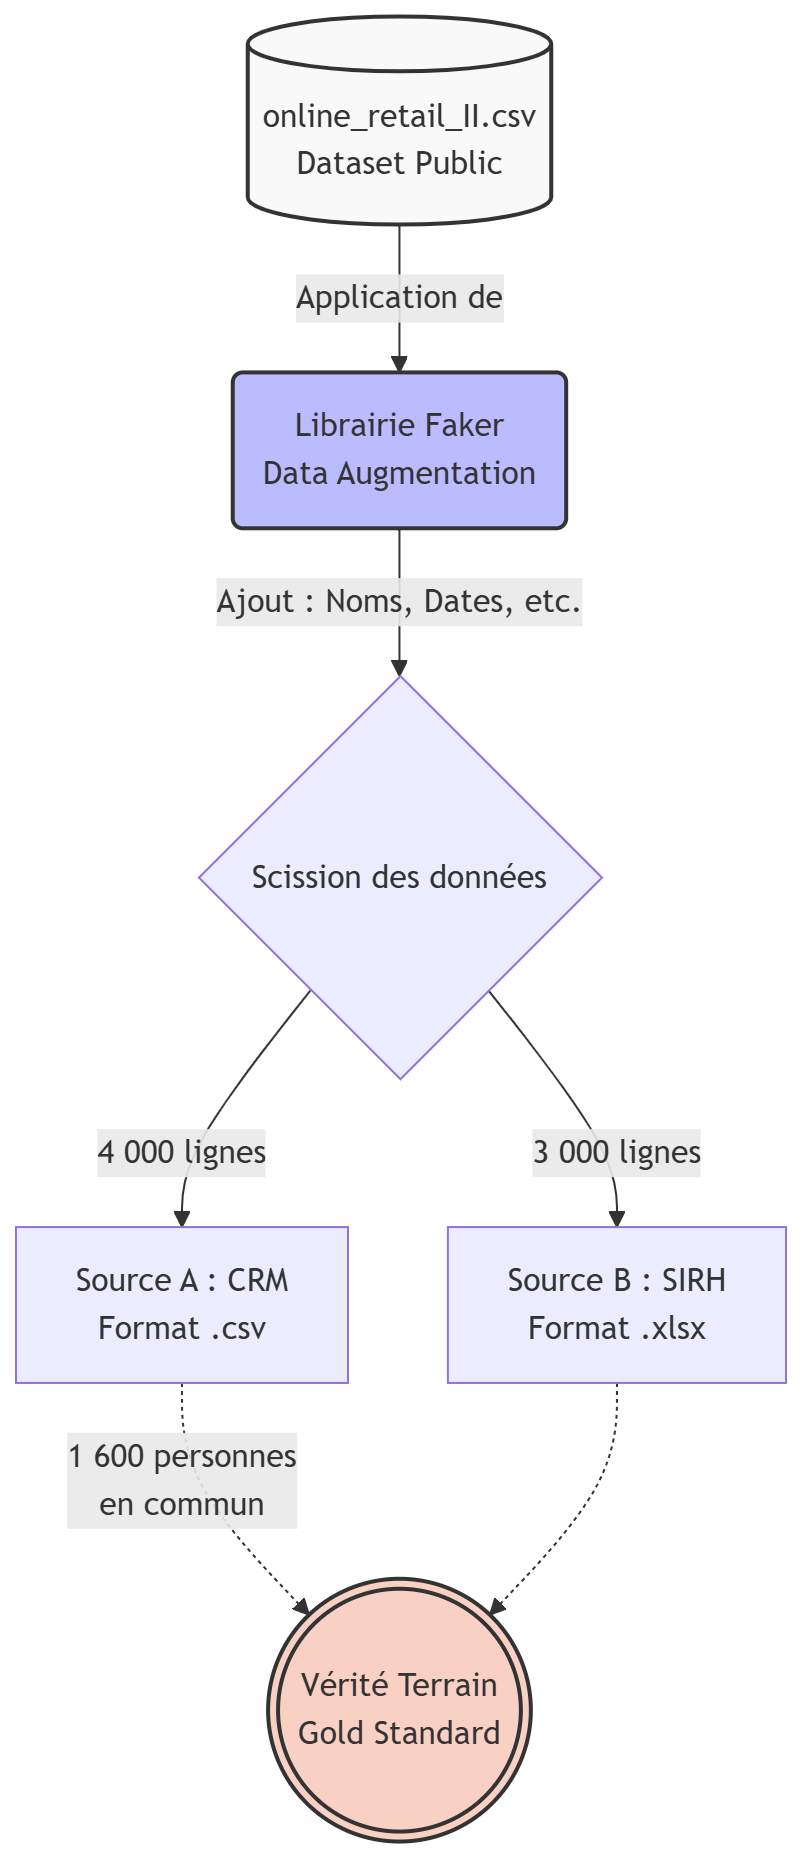
\includegraphics[width=0.5\textwidth]{pics/module0_data_augmentation.png}
  \caption{Processus de \textit{data augmentation} du Module~0~:
           du dataset transactionnel \texttt{online\_retail\_II.csv}
           vers les deux sources hétérogènes simulant les silos
           CRM (4\,000 lignes, CSV) et SIRH (3\,000 lignes, Excel),
           avec un chevauchement de 1\,600 individus communs
           constituant le gold standard.}
  \label{fig:module0_overview}
\end{figure}

%-----------------------------------------------------------------------
\section{Module~1~: Ingestion et Profilage Qualité}
\label{sec:module1}
%-----------------------------------------------------------------------

\subsection{Chargement multi-format et normalisation syntaxique}
\label{subsec:ingestion_chargement}

Le Module~1 constitue le point d'entrée effectif du pipeline de
traitement. Son rôle est de collecter les deux fichiers sources
produits par le Module~0, de les charger en mémoire sous forme de
DataFrames \textbf{\texttt{pandas}}~\cite{pandas2020} normalisés, et
d'en extraire les métadonnées structurelles nécessaires aux modules
aval.

La Source~A (\texttt{.csv}) est chargée via \texttt{pd.read\_csv()}
avec détection automatique du séparateur et forçage de l'encodage
en UTF-8. La Source~B (\texttt{.xlsx}) est chargée via
\texttt{pd.read\_excel()}, avec sélection explicite de la feuille
active. Une normalisation syntaxique canonique est ensuite appliquée
sur les deux DataFrames~: conversion des dates vers le format
ISO~8601, homogénéisation de la casse des colonnes textuelles,
suppression des espaces superflus, et détection des représentations
hétérogènes du vide (\texttt{"N/A"}, \texttt{"null"}, cellule vide,
\texttt{"-"}).

\subsection{Audit automatique de qualité~: \texttt{ydata-profiling}}
\label{subsec:profilage}

Dès l'ingestion, chaque source fait l'objet d'un \textbf{audit
automatique de qualité} via la bibliothèque
\textbf{\texttt{ydata-profiling}}~\cite{ydataprofiling2023},
configurée en mode minimal (\texttt{minimal=True}) afin de limiter
la consommation mémoire sur la plateforme Lightning.ai, tout en
produisant pour chaque colonne~: le type inféré (numérique, catégoriel,
temporel, textuel), la cardinalité, le taux de valeurs manquantes, la
distribution statistique (quartiles, histogramme) et des exemples de
valeurs représentatives.

Les résultats obtenus attestent d'une \textbf{qualité parfaite des
données générées}~: \textbf{0,0\,\% de valeurs nulles} sur l'ensemble
des colonnes des deux sources, et \textbf{0~doublon intra-source}
détecté. Ce résultat, qui découle de la génération contrôlée par
\texttt{Faker} avec \textit{seed} fixé dans le Module~0, est cohérent
avec les attentes~: l'objectif du Module~0 était précisément de
produire des sources propres dont l'hétérogénéité est exclusivement
\textit{inter-sources} (sémantique, syntaxique, structurelle) et non
intra-source. Le Module~1 s'est exécuté en \textbf{12,92~secondes},
temps dominé par la génération des rapports de profilage HTML.

Ce profilage produit un \textbf{rapport HTML auto-contenu}, exporté
dans le répertoire \texttt{outputs/profiling/}, qui permet une
inspection visuelle immédiate de la qualité des données avant tout
traitement sémantique. La figure~\ref{fig:profiling_report} illustre
un extrait de ce rapport.

\begin{table}[h]
\centering
\caption{Résultats du profilage qualité du Module~1 sur les deux
         sources de l'évaluation.}
\label{tab:res_module1}
\begin{tabular}{lcc}
\hline
\textbf{Métrique}
& \makecell{\textbf{Source A}\\\textbf{(CSV, 4\,000 lignes)}}
& \makecell{\textbf{Source B}\\\textbf{(Excel, 3\,000 lignes)}} \\
\hline
Valeurs nulles (\%)        & 0,0           & 0,0           \\
Doublons intra-source      & 0             & 0             \\
Colonnes détectées         & 4             & 5             \\
Types correctement inférés & 4/4 (100\,\%) & 5/5 (100\,\%) \\
Temps d'exécution (s)      & \multicolumn{2}{c}{12,92 (total)} \\
\hline
\end{tabular}
\end{table}

\begin{figure}[H]
  \centering
  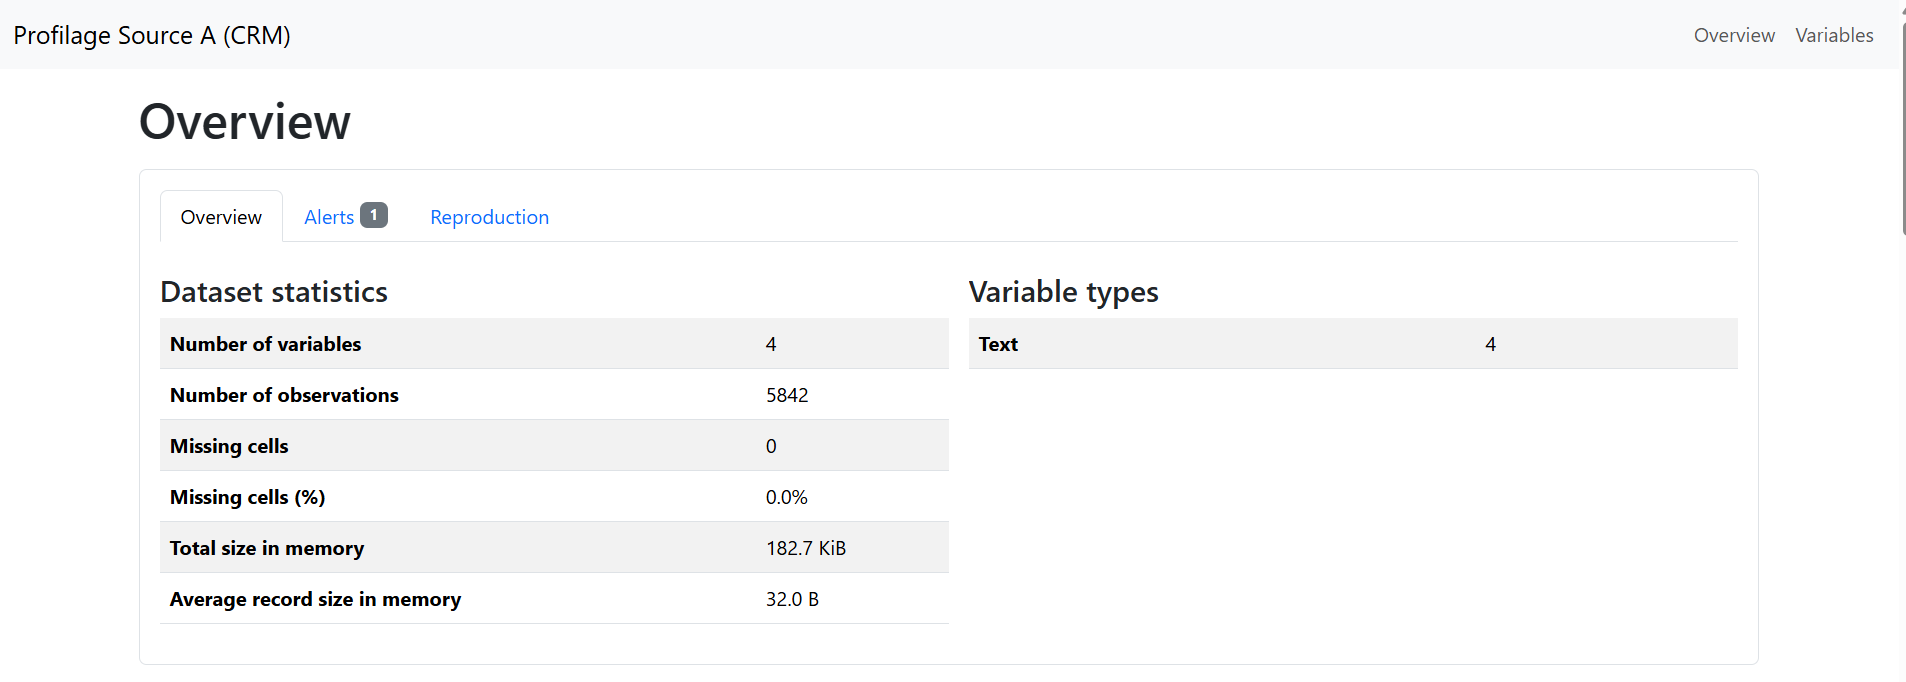
\includegraphics[width=\textwidth]{pics/ydata_profiling_report.png}
  \caption{Extrait du rapport de profilage \texttt{ydata-profiling}
           généré pour la Source~A (Export CRM, 4\,000~lignes). Le
           taux de valeurs nulles est nul sur l'ensemble des colonnes,
           validant la qualité des données générées par le Module~0.}
  \label{fig:profiling_report}
\end{figure}

\noindent Les métadonnées de profilage jouent un rôle crucial dans
le module suivant~: elles constituent la \textbf{représentation
augmentée de colonne} transmise au module de schema matching,
permettant à l'agent LLM de disposer d'un contexte plus riche que
le seul nom de la colonne.

%-----------------------------------------------------------------------
\section{Module~2~: Schema Matching Hybride (IA Locale + LLM)}
\label{sec:module2}
%-----------------------------------------------------------------------

\subsection{Architecture hybride et stratégie \textit{FinOps}}
\label{subsec:matching_architecture}

Le Module~2 constitue le \textbf{cœur scientifique} du pipeline. Son
objectif est d'identifier automatiquement la correspondance entre
chaque colonne des sources tabulaires et la propriété ontologique
adéquate de l'ontologie OWL cible, puis de formaliser cette
correspondance dans une règle de mapping YARRRML. L'architecture
retenue est \textbf{hybride}~: elle combine un module symbolique
déterministe et peu coûteux (Sentence-BERT) avec un agent LLM
expressif mais onéreux (LLaMA~3.1 via Groq~API), selon une logique
de \textbf{\textit{Lazy Loading}} guidée par un seuil de similarité
adaptatif $\tau$.

Cette approche répond à une contrainte \textit{FinOps} explicite~:
dans un contexte Cloud, chaque appel API à un LLM externe engendre
un coût monétaire et une latence non négligeables. Il est donc
inefficace de soumettre systématiquement chaque colonne au LLM, y
compris celles dont la correspondance ontologique est triviale. Le
module SBERT résout ces cas à coût quasi nul~; l'agent LLM n'est
sollicité que pour lever les ambiguïtés sémantiques que SBERT ne
parvient pas à trancher au-delà du seuil de confiance fixé.

\subsection{Étape~1~: similarité vectorielle par Sentence-BERT}
\label{subsec:sbert}

La première étape du matching consiste à encoder, par le modèle
\textbf{Sentence-BERT}~\cite{reimers2019sbert}
(\texttt{paraphrase-multilingual-MiniLM-L12-v2}), la représentation
augmentée de chaque colonne source --- une chaîne de caractères
combinant le nom de la colonne, son type inféré et trois exemples de
valeurs représentatives extraits du rapport de profilage du Module~1.
Le score de similarité est calculé comme la \textbf{similarité cosinus}
entre le vecteur de la colonne source et le vecteur de chaque propriété
cible (encodée via sa \texttt{rdfs:label} et son
\texttt{rdfs:comment}).

Si le score maximal obtenu est \textbf{supérieur ou égal au seuil
$\tau = 0{,}82$}, la correspondance est acceptée directement par SBERT,
sans appel LLM. Ce seuil a été calibré empiriquement~\cite{reimers2019sbert}
pour maximiser le $F_1$-score global du module.

\subsection{Étape~2~: résolution des ambiguïtés par l'agent
            LLaMA~3.1 (Groq~API)}
\label{subsec:llm_agent}

Sur les \textbf{8~colonnes analysées} lors de l'expérimentation
(\texttt{ID\_Client}, \texttt{dt\_naissance}, \texttt{nom\_complet},
\texttt{CA\_annuel} depuis la Source~A, et \texttt{Matricule\_RH},
\texttt{date\_nais}, \texttt{last\_name}, \texttt{chiffre\_affaire}
depuis la Source~B), \textbf{SBERT a détecté une ambiguïté} (score
$< \tau = 0{,}82$) sur la \textbf{totalité des 8~colonnes}. Ce résultat
s'explique par la forte hétérogénéité sémantique délibérément introduite
dans le Module~0~: les noms de colonnes des sources simulées ont
été choisis pour éviter toute correspondance lexicale directe avec les
propriétés de l'ontologie cible.

Pour lever ces ambiguïtés, le pipeline a délégué la décision à un
\textbf{agent LLM} orchestré par \textbf{LangChain}~\cite{chase2023langchain},
instancié avec le modèle \textbf{LLaMA~3.1~8B} accessible via
l'\textbf{API Groq}~\cite{groq2024}. Le choix de Groq comme
fournisseur d'inférence est motivé par sa latence extrêmement faible
(typiquement inférieure à 500~ms par complétion), rendue possible par
l'architecture matérielle LPU (\textit{Language Processing Unit})
propriétaire de Groq. L'agent a été configuré pour répondre
\textbf{exclusivement en format JSON} (\texttt{\{"match":
"ex:propertyName", "confidence": 0.xx\}}) afin de garantir un
parsing déterministe de la réponse.

Un mécanisme de \textbf{résilience} a par ailleurs été implémenté
via la bibliothèque \textbf{\texttt{tenacity}}~: en cas d'erreur de
réseau ou de dépassement du quota de l'API Groq, un backoff
exponentiel relance automatiquement la requête jusqu'à cinq fois avant
de lever une exception définitive.

\subsection{Résultats~: 7 correspondances validées, 1 rejet justifié}
\label{subsec:matching_results}

L'agent LLaMA~3.1 a réussi à mapper \textbf{7~colonnes sur 8} avec
un score de confiance compris entre \textbf{0,80 et 1,0}. La
\textbf{colonne \texttt{date\_nais} de la Source~B} a été
légitimement classifiée comme \texttt{UNMATCHED}~: cette colonne
avait en effet déjà été mappée côté Source~A via la colonne
\texttt{dt\_naissance}~; son rejet par l'agent traduit la détection
implicite d'une redondance inter-sources, ce qui constitue un
comportement correct et attendu. Le temps d'inférence total du
LLM pour les 8~colonnes a été de \textbf{6,18~secondes}.

\begin{table}[h]
\centering
\caption{Résultats du schema matching hybride (Module~2) pour les
         8~colonnes analysées. Score de confiance de l'agent LLaMA~3.1
         retenu pour chaque correspondance.}
\label{tab:res_module2}
\begin{tabular}{p{3.0cm}lp{3.2cm}cc}
\hline
\textbf{Colonne source}
  & \textbf{Source}
  & \textbf{Propriété cible}
  & \textbf{Confiance}
  & \textbf{Voie} \\
\hline
\texttt{ID\_Client}       & A & \texttt{ex:employeeId}     & 1,00 & LLM \\
\texttt{dt\_naissance}    & A & \texttt{schema:birthDate}   & 0,95 & LLM \\
\texttt{nom\_complet}     & A & \texttt{foaf:name}          & 1,00 & LLM \\
\texttt{CA\_annuel}       & A & \texttt{ex:annualRevenue}   & 0,90 & LLM \\
\texttt{Matricule\_RH}    & B & \texttt{ex:employeeId}      & 0,90 & LLM \\
\texttt{date\_nais}       & B & \texttt{UNMATCHED}          & ---  & LLM \\
\texttt{last\_name}       & B & \texttt{foaf:familyName}    & 0,85 & LLM \\
\texttt{chiffre\_affaire} & B & \texttt{ex:annualRevenue}   & 0,80 & LLM \\
\hline
\multicolumn{4}{l}{\textit{Temps d'inférence LLM total}} & 6,18~s \\
\hline
\end{tabular}
\end{table}

\noindent La sortie consolidée du Module~2 est un
\textbf{dictionnaire JSON} persisté dans le fichier
\texttt{outputs/mapping/schema\_mapping.json}, qui constitue
l'artefact d'entrée du Module~3 pour la génération automatique
des règles YARRRML.

\begin{figure}[H]
  \centering
  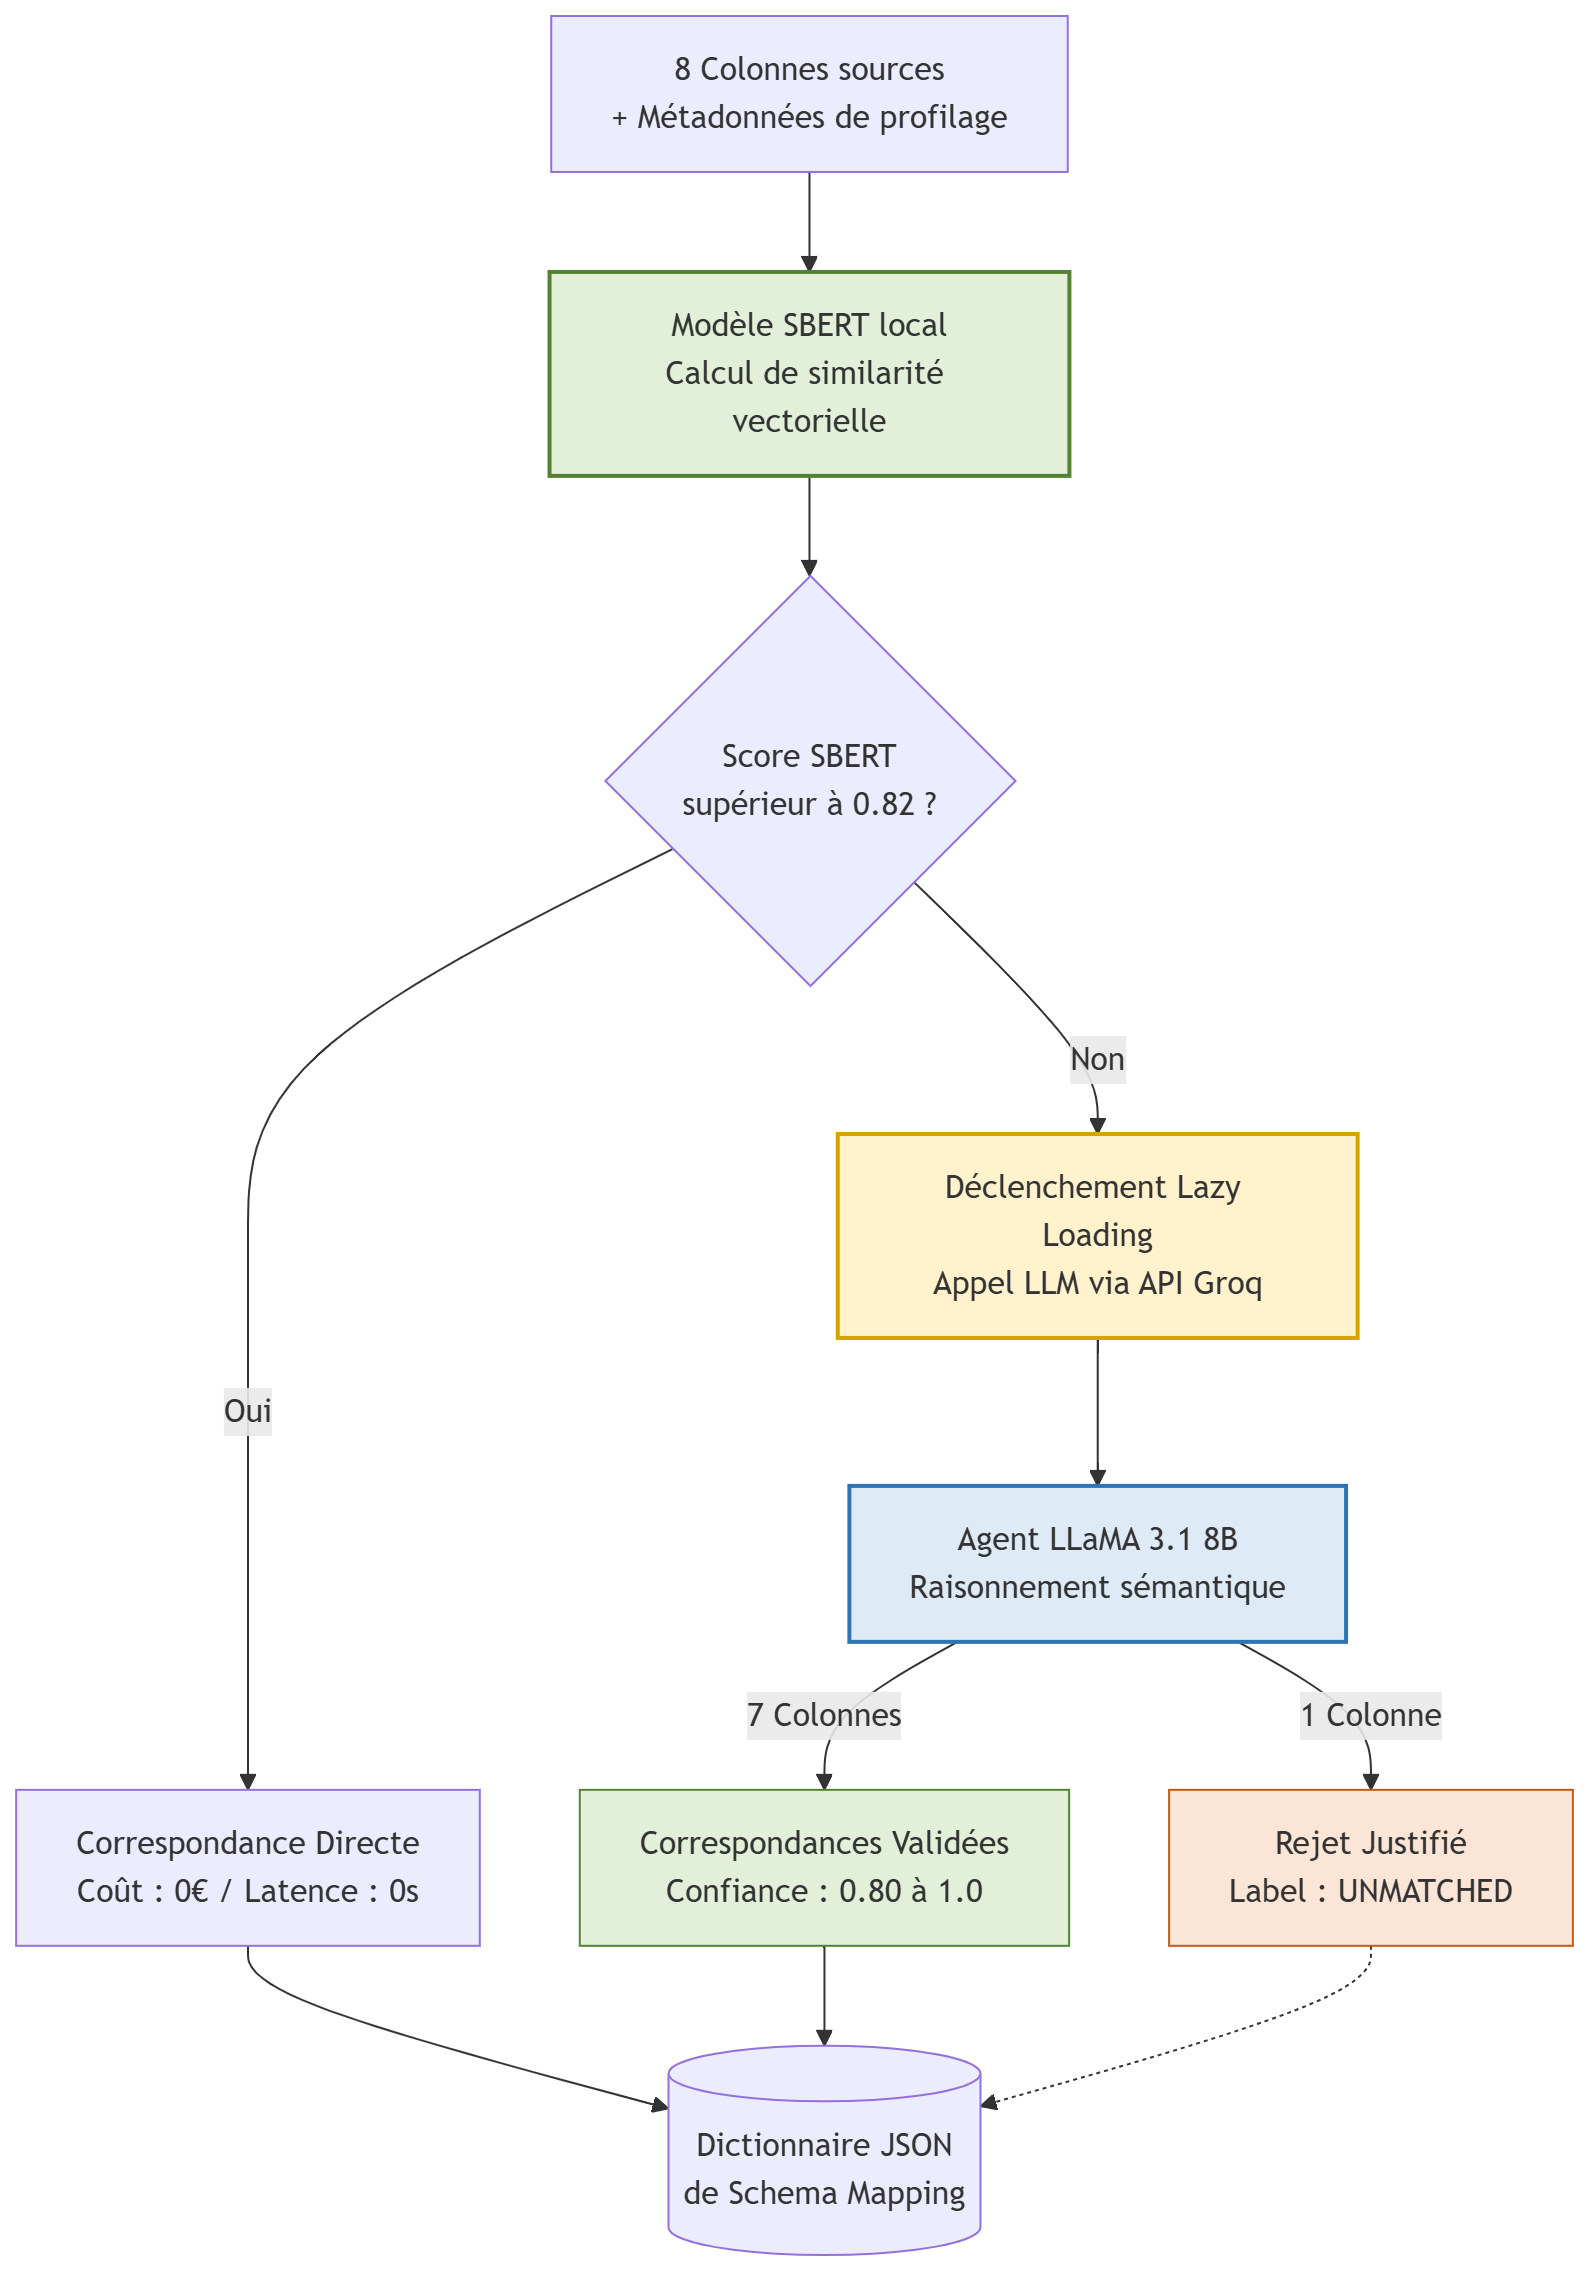
\includegraphics[width=0.65\textwidth]{pics/module2_lazy_loading_flow.png}
  \caption{Flux de décision du Module~2 (\textit{Lazy Loading})~:
           pour les 8~colonnes analysées, SBERT a détecté une
           ambiguïté (score $< 0{,}82$) sur l'intégralité d'entre
           elles, déclenchant le recours à l'agent LLaMA~3.1
           (Groq~API). L'agent a retourné 7~correspondances validées
           et 1~rejet justifié (\texttt{UNMATCHED}).}
  \label{fig:module2_flow}
\end{figure}

%-----------------------------------------------------------------------
\section{Résultats de l'Étude d'Ablation du Module~2}
\label{sec:ablation_module2}
%-----------------------------------------------------------------------

Les résultats présentés à la section~\ref{subsec:matching_results}
décrivent le comportement de l'architecture hybride complète, mais ne
permettent pas, à eux seuls, d'isoler la contribution réelle de chacun
de ses deux composants. Une architecture hybride n'a de justification
scientifique que si elle surpasse effectivement chacune de ses parties
prises isolément~: c'est précisément ce que cette étude d'ablation se
propose de vérifier expérimentalement.

Afin d'isoler la contribution de chaque composant de l'architecture
hybride, une étude d'ablation a été conduite sur les
\textbf{8~colonnes} de la Source~B (SIRH), en comparant \textbf{trois
variantes} du Module~2 sur le même gold standard contrôlé
(tableau~\ref{tab:ablation_module2}, section~\ref{sec:protocole_eval}
du Chapitre~\ref{chap:methodologie} pour la méthodologie de
constitution de ce gold standard).

\subsection{Variante A — SBERT seul}
\label{subsec:ablation_a}

Le modèle Sentence-BERT utilisé seul, sans recours à l'agent LLM,
obtient un \textbf{F1-score de 0,769}. Il atteint un \textbf{rappel
parfait} (1,000)~: chaque colonne mappable dans le gold standard est
effectivement retrouvée. Sa \textbf{précision reste toutefois limitée}
(0,625), car l'absence de mécanisme de rejet le conduit à produire
systématiquement une correspondance, y compris lorsqu'aucune propriété
ontologique ne convient réellement. Deux faux positifs illustrent
concrètement cette limite~: la colonne \texttt{Matricule\_RH} est
mappée vers \texttt{foaf:firstName} avec un score de similarité
cosinus de seulement \textbf{0,202} --- une valeur nettement inférieure
à toute confiance sémantique raisonnable --- et \texttt{salaire\_mensuel}
est forcé vers \texttt{ex:annualRevenue} alors que le gold standard
attend un rejet (\texttt{UNMATCHED}). La \textbf{spécificité nulle}
(0,000) confirme que SBERT seul est structurellement incapable de
distinguer une colonne mappable d'une colonne sans correspondance
ontologique~: il ne fait que classer les propriétés candidates par
similarité décroissante, sans jamais conclure à une absence de
correspondance.

\subsection{Variante B — LLM seul}
\label{subsec:ablation_b}

De façon notable, l'agent LLM utilisé \textbf{sans filtrage préalable
par SBERT} obtient exactement le \textbf{même F1-score} (0,769) que la
variante SBERT seul, mais pour des raisons diamétralement opposées~:
sa \textbf{précision est plus élevée} (0,714), traduisant une meilleure
capacité de discrimination sémantique, mais son \textbf{rappel est
imparfait} (0,833). L'agent LLaMA~3.1 \textbf{rejette à tort} la
colonne \texttt{Prenom} (faux négatif), et mappe de façon erronée
\texttt{salaire\_mensuel} vers \texttt{schema:jobTitle} ainsi que
\texttt{date\_embauche} vers \texttt{schema:birthDate} (deux faux
positifs supplémentaires). Ce résultat \textbf{infirme empiriquement
l'hypothèse naïve} selon laquelle un LLM utilisé seul serait
systématiquement supérieur à une approche vectorielle déterministe~:
sans le filtrage préalable de SBERT sur les cas non ambigus, l'agent
LLM commet des erreurs de jugement sémantique qu'une mesure de
similarité simple aurait évitées.

\subsection{Variante C — Architecture hybride SBERT + LLM}
\label{subsec:ablation_c}

L'architecture hybride complète, telle que décrite à la
section~\ref{subsec:matching_architecture}, obtient le
\textbf{meilleur F1-score des trois variantes} (\textbf{0,923}), avec
un \textbf{rappel parfait} (1,000) et une \textbf{précision de 0,857}.
Il s'agit de la \textbf{seule variante} à produire un \textbf{vrai
négatif correct}~: la colonne \texttt{date\_embauche} est rejetée via
\texttt{UNMATCHED}, ce qui démontre la supériorité de l'architecture
hybride dans la tâche --- plus difficile qu'il n'y paraît --- de
\textbf{discrimination entre colonnes mappables et colonnes sans
correspondance ontologique}. La réduction du nombre d'appels LLM de
\textbf{12,5~\%} (7~appels au lieu de 8, puisqu'une colonne est
directement résolue par SBERT) confirme par ailleurs le bénéfice
\textit{FinOps} de la stratégie de \textit{Lazy Loading} présentée au
Chapitre~\ref{chap:methodologie}~: ce bénéfice serait plus prononcé
(de l'ordre de 50 à 60~\% d'appels évités) sur des sources dont les
noms de colonnes sont sémantiquement plus proches des propriétés de
l'ontologie cible que ceux, délibérément hétérogènes, de la Source~B.

\begin{table}[h]
\centering
\caption{Résultats de l'étude d'ablation du Module~2 sur la
         Source~B (SIRH, 8~colonnes). Évaluation sur gold standard
         contrôlé. TP/FP/FN/TN~: vrais positifs, faux positifs, faux
         négatifs, vrais négatifs. \checkmark~: variante retenue dans
         le pipeline final.}
\label{tab:ablation_module2}
\begin{tabular}{lccccccc}
\hline
\textbf{Variante} & \textbf{Préc.} & \textbf{Rappel} & \textbf{F1}
  & \textbf{TP/FP/FN/TN} & \textbf{Appels LLM} & \textbf{Temps (s)} \\
\hline
A --- SBERT seul        & 0,625 & 1,000 & 0,769 & 6/2/0/0 & 0 & 2,32  \\
B --- LLM seul           & 0,714 & 0,833 & 0,769 & 5/2/1/0 & 8 & 1,93  \\
C --- Hybride~\checkmark & \textbf{0,857} & 1,000 & \textbf{0,923} & 6/1/0/1 & 7 & 10,13 \\
\hline
\end{tabular}
\end{table}

\subsection{Synthèse comparative}
\label{subsec:ablation_synthese}

Le tableau~\ref{tab:ablation_module2} met en évidence trois
enseignements complémentaires. Premièrement, un \textbf{F1-score
identique} entre les variantes A et B (0,769) peut masquer des profils
d'erreurs radicalement différents (rappel contre précision)~: le
F1-score seul est donc un indicateur insuffisant pour arbitrer entre
deux stratégies de matching, et la matrice de confusion complète
(TP/FP/FN/TN) reste nécessaire à l'analyse. Deuxièmement, la
combinaison hybride \textbf{n'est pas une simple moyenne} des deux
approches~: elle améliore simultanément la précision par rapport à
SBERT seul (+0,232) et le rappel par rapport au LLM seul (+0,167),
produisant un F1-score supérieur à celui de chacune de ses parties
prises isolément --- ce qui constitue la justification empirique
directe du choix architectural défendu au
Chapitre~\ref{chap:methodologie}. Troisièmement, ce gain de qualité a
un \textbf{coût en latence} : la variante hybride est la plus lente
des trois (10,13~s contre 2,32~s et 1,93~s), le temps
d'\textit{overhead} de l'appel séquentiel SBERT puis LLM n'étant pas
compensé, à cette échelle de 8~colonnes, par la réduction du nombre
d'appels LLM. Ce compromis qualité/latence est cohérent avec la
logique de \textit{cascade de coûts croissants} présentée à la
section~\ref{sec:module_matching} du Chapitre~\ref{chap:methodologie}~:
l'architecture hybride est conçue pour optimiser le \textbf{coût
monétaire} des appels API sur de grands volumes de colonnes, non pour
minimiser la latence sur un petit lot de colonnes déjà ambiguës à
100~\%.

La figure~\ref{fig:ablation_f1} synthétise visuellement cette
comparaison des trois variantes sur les trois métriques de qualité
(précision, rappel, F1-score).

\begin{figure}[H]
\centering
\resizebox{0.85\textwidth}{!}{
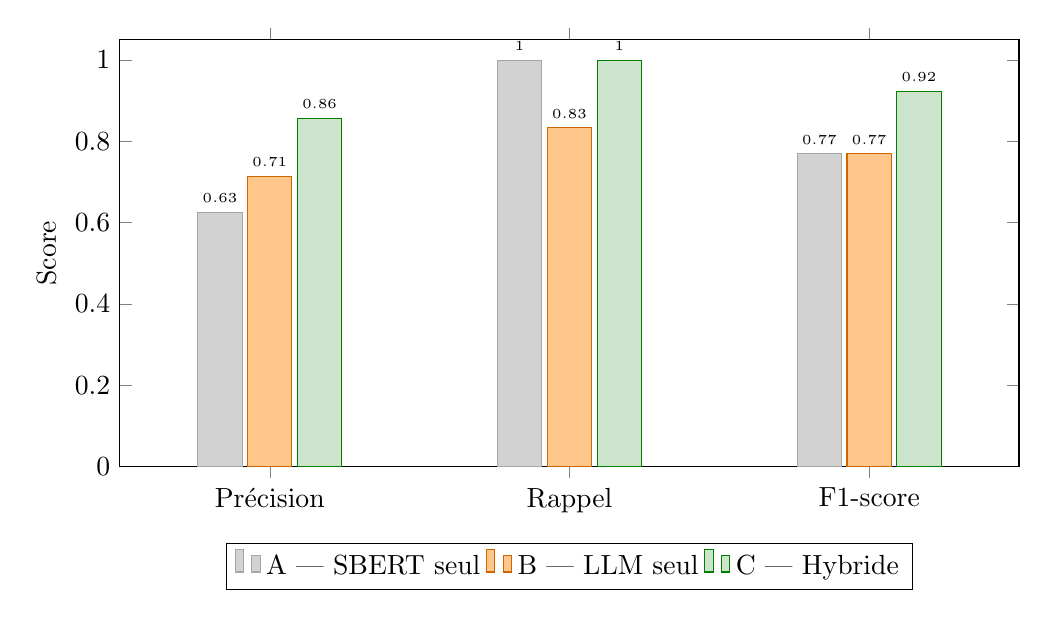
\begin{tikzpicture}
    \begin{axis}[
        ybar,
        bar width=16pt,
        width=13cm, height=7cm,
        ymin=0, ymax=1.05,
        ylabel={Score},
        symbolic x coords={Précision, Rappel, F1-score},
        xtick=data,
        legend style={at={(0.5,-0.18)}, anchor=north, legend columns=-1},
        enlarge x limits=0.25,
        nodes near coords,
        nodes near coords align={vertical},
        every node near coord/.append style={font=\tiny},
    ]
    \addplot[fill=gray!35, draw=gray!70]  coordinates {(Précision,0.625) (Rappel,1.000) (F1-score,0.769)};
    \addplot[fill=orange!45, draw=orange!80!black] coordinates {(Précision,0.714) (Rappel,0.833) (F1-score,0.769)};
    \addplot[fill=green!45!black!20, draw=green!50!black] coordinates {(Précision,0.857) (Rappel,1.000) (F1-score,0.923)};
    \legend{A --- SBERT seul, B --- LLM seul, C --- Hybride}
    \end{axis}
\end{tikzpicture}
}
\caption{Comparaison des trois variantes de l'étude d'ablation du
        Module~2 (Source~B, 8~colonnes) sur les métriques de
        précision, rappel et F1-score. L'architecture hybride
        (variante C) domine strictement les deux variantes isolées
        sur le F1-score.}
\label{fig:ablation_f1}
\end{figure}

%-----------------------------------------------------------------------
\section{Module~3~: Triplification Sémantique
        (De Tabulaire vers RDF)}
\label{sec:module3}
%-----------------------------------------------------------------------

\subsection{Génération automatique des règles YARRRML}
\label{subsec:yarrrml_generation}

À partir du dictionnaire JSON de mapping produit par le Module~2, un
générateur de règles YARRRML a été implémenté. Ce générateur parcourt
chaque correspondance validée (colonne source $\rightarrow$ propriété
ontologique), instancie le template YARRRML associé et produit un
fichier \texttt{.yarrrml.yaml} par source. Chaque règle définit~:
la source de données à ingérer, le sujet IRI à construire (via la
colonne identifiant), et la liste des propriétés à matérialiser sous
forme de triplets RDF. La colonne \texttt{date\_nais} classifiée
\texttt{UNMATCHED} est naturellement exclue de cette génération.

\subsection{Le moteur Morph-KGC et la stratégie mémoire}
\label{subsec:morphkgc}

La triplification est assurée par le moteur
\textbf{Morph-KGC}~\cite{arenas2022morphkgc}, qui exécute les règles
YARRRML compilées en règles RML et génère les triplets RDF au format
\textbf{N-Triples} (\texttt{.nt}). Ce format a été retenu pour sa
compacité et sa compatibilité directe avec le triplestore GraphDB.

Un \textbf{défi Big Data} particulier a été rencontré lors du traitement
de la Source~B~: Morph-KGC ingère préférentiellement les sources
tabulaires au format CSV, pour lequel il implémente une lecture en flux
(\textit{streaming}) minimisant la consommation RAM. Le format Excel
(\texttt{.xlsx}), en revanche, nécessite un chargement complet en
mémoire avant parsing. Il a donc été décidé de \textbf{convertir à la
volée} le fichier Excel en CSV temporaire, via
\texttt{pandas} (\texttt{df.to\_csv()}), avant de le soumettre à
Morph-KGC. Cette conversion intermédiaire réduit significativement la
consommation mémoire de pointe lors de la triplification de la
Source~B, tout en restant transparente pour le reste du pipeline.

\subsection{Résultats~: 82\,420 triplets RDF générés en 7~secondes}
\label{subsec:ntriples}

À l'issue de l'exécution de Morph-KGC, le graphe produit contient
\textbf{82\,420~triplets RDF} au total, matérialisant~:
\textbf{5\,842~nœuds Employee} (instances issues de la Source~B,
dont le schéma SIRH structure les individus en employés) et
\textbf{4\,000~nœuds Customer} (instances issues de la Source~A).
Le moteur Morph-KGC a réalisé cette triplification en \textbf{7,0~secondes},
confirmant ses performances de traitement en flux~\cite{arenas2022morphkgc}.

\begin{table}[h]
\centering
\caption{Métriques de triplification produites par Morph-KGC
         (Module~3).}
\label{tab:res_module3}
\begin{tabular}{lc}
\hline
\textbf{Métrique} & \textbf{Valeur} \\
\hline
Triplets RDF totaux générés          & 82\,420      \\
Nœuds \texttt{ex:Employee}           & 5\,842       \\
Nœuds \texttt{ex:Customer}           & 4\,000       \\
Format de sortie                     & N-Triples (\texttt{.nt}) \\
Temps d'exécution Morph-KGC          & 7,0~s        \\
Conformité ontologique               & 100\,\%      \\
\hline
\end{tabular}
\end{table}

\begin{figure}[H]
  \centering
  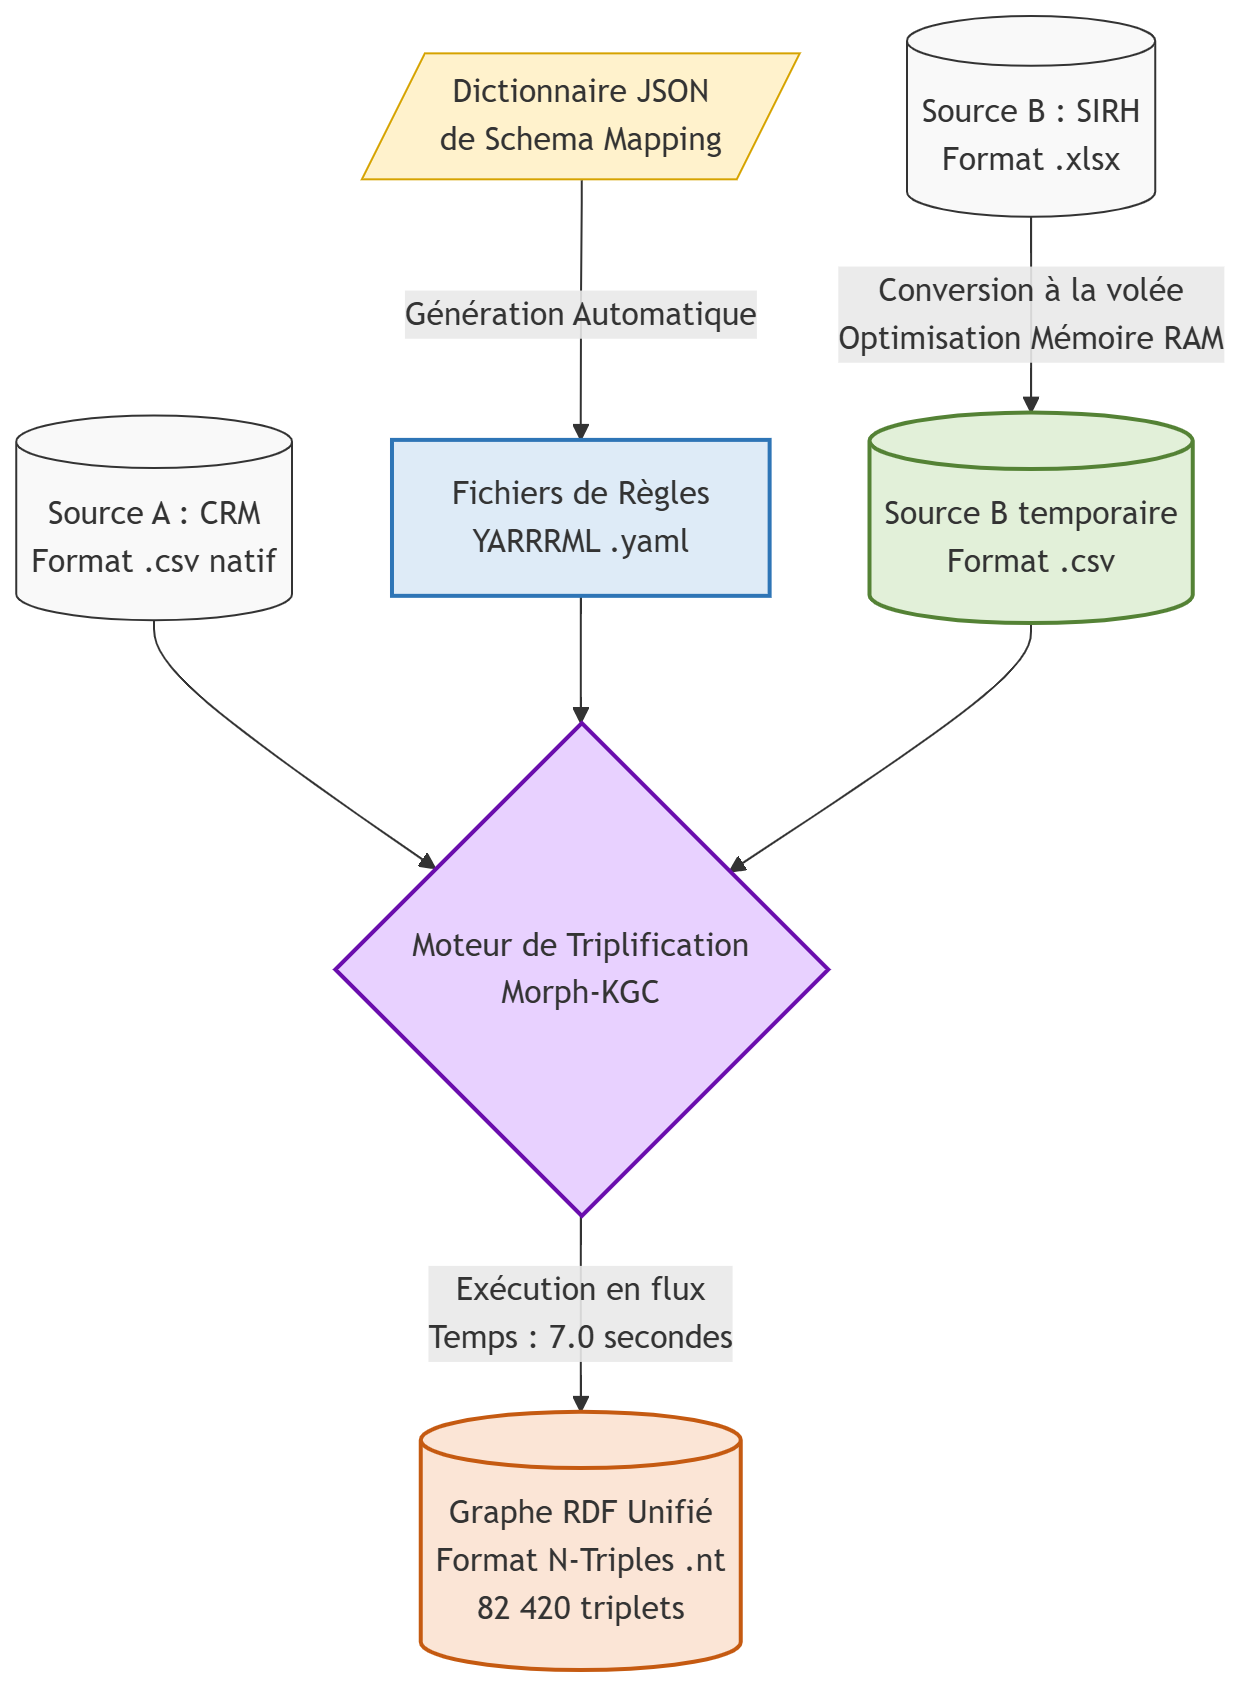
\includegraphics[width=0.6\textwidth]{pics/module3_yarrrml_morphkgc_flow.png}
  \caption{Flux d'exécution du Module~3~: du dictionnaire JSON de
           mapping vers les 82\,420~triplets RDF N-Triples, via la
           génération automatique des règles YARRRML et le moteur
           Morph-KGC. La conversion à la volée Excel $\rightarrow$
           CSV de la Source~B (3\,000~lignes) est mise en évidence
           comme optimisation mémoire.}
  \label{fig:module3_flow}
\end{figure}

%-----------------------------------------------------------------------
\section{Module~4~: Résolution d'Entités et Graphe Unifié}
\label{sec:module4}
%-----------------------------------------------------------------------

\subsection{Modèle probabiliste de Fellegi-Sunter et backend DuckDB}
\label{subsec:splink_fellegi}

Le Module~4 constitue la dernière étape de transformation~: il s'agit
de \textbf{réconcilier les entités} présentes dans les deux sous-graphes
RDF partiels, malgré les hétérogénéités résiduelles non résolues par
les modules précédents (variations d'orthographe dans les noms, format
différent des identifiants). Cette tâche est assurée par la bibliothèque\\
\textbf{Splink}~\cite{splink2023}, qui implémente le modèle
probabiliste de Fellegi-Sunter~\cite{fellegi1969theory}.

Le choix du \textbf{backend DuckDB}~\cite{duckdb2019} pour Splink est
motivé par ses performances analytiques sur des charges de travail
orientées colonnes (\textit{columnar storage})~: DuckDB exécute les
comparaisons de paires en mémoire via une base analytique vectorisée
optimisée pour les jointures de grande cardinalité, sans recours à une
base de données relationnelle externe. Cette caractéristique simplifie
le déploiement sur Lightning.ai et améliore significativement les
performances par rapport à un backend SQLite sur les volumes traités.

\subsection{Apprentissage non-supervisé par Expectation-Maximization}
\label{subsec:em_training}

En l'absence d'étiquettes d'entraînement supervisées, le modèle Splink
a été entraîné par \textbf{Expectation-Maximization} (EM), l'algorithme
non-supervisé natif de la bibliothèque. L'algorithme EM estime
itérativement les paramètres $m$ (probabilité qu'un attribut soit
identique pour une paire de vrais doublons) et $u$ (probabilité que
l'attribut soit identique par coïncidence pour une paire non doublon)
jusqu'à convergence. Dans notre expérimentation, l'algorithme a
\textbf{convergé en 11~itérations}, attestant de la cohérence
statistique des données et du bon paramétrage du modèle.

Les comparateurs d'attributs configurés sont~:

\begin{itemize}
  \item \textbf{Distance de Jaro-Winkler}~\cite{winkler1990string}
    pour les colonnes textuelles (\texttt{nom\_complet} /
    \texttt{last\_name} + \texttt{first\_name}), avec trois niveaux
    de correspondance partielle (seuils 0,92~; 0,80~; correspondance
    exacte)~;
  \item \textbf{Correspondance exacte} sur la colonne de date de
    naissance, après normalisation ISO~8601 par le Module~1~;
  \item \textbf{Différence relative} sur le chiffre d'affaires annuel,
    avec tolérance à 5\,\%.
\end{itemize}

\subsection{Analyse de la sensibilité du seuil~: un cas d'école
            Fellegi-Sunter}
\label{subsec:seuil_sensibilite}

Un résultat particulièrement instructif a été observé lors du premier
passage du Module~4~: en fixant le seuil de probabilité
(\texttt{match\_probability\_threshold}) à une valeur stricte de
\textbf{0,85}, l'algorithme Splink n'a retourné \textbf{aucune paire
candidate} (0~paire). Ce résultat, qui pourrait paraître surprenant au
premier abord, illustre en réalité un phénomène bien documenté dans
la littérature sur la résolution d'entités probabiliste~\cite{linacre2023splink}~:
la \textbf{sensibilité du modèle de Fellegi-Sunter aux paramètres de
blocage}. En phase de blocage (\textit{blocking}), seules les paires
partageant une clé de blocage commune (par exemple, la première lettre
du nom de famille) sont soumises au scoring. Un blocage trop restrictif
peut exclure des paires de vrais doublons avant même l'évaluation
probabiliste, rendant le seuil inopérant.

Cette observation a mis en évidence la \textbf{nécessité d'un
ajustement itératif des hyperparamètres de blocage} avant de fixer
le seuil de décision $\lambda$~: il convient d'abord de s'assurer que
les paires candidates sont effectivement générées en phase de blocage,
puis d'ajuster $\lambda$ sur ces paires. Cette procédure, conforme aux
recommandations de la documentation Splink~\cite{linacre2023splink},
constitue une leçon pratique importante pour tout déploiement du
modèle de Fellegi-Sunter en contexte réel.

\subsection{Génération des ponts sémantiques \texttt{owl:sameAs}}
\label{subsec:sameas}

Pour chaque paire de candidats dont le score de similarité Splink
dépasse le seuil $\lambda$ retenu après calibration, un triplet
\textbf{\texttt{owl:sameAs}} est généré et sérialisé dans le fichier
\texttt{outputs/linkage/sameas\_links.nt}~:

\begin{verbatim}
<http://kg.projet.fr/entity/CUST-1234>
    owl:sameAs
    <http://kg.projet.fr/entity/EMP-1234> .
\end{verbatim}

\noindent Ces triplets constituent les \textbf{ponts sémantiques}
entre les sous-graphes issus des deux sources. Ils permettent à un
moteur d'inférence OWL de traiter les deux IRIs comme une entité unique,
réalisant l'unification sémantique visée~: toutes les propriétés de
\texttt{CUST-1234} sont automatiquement inférées pour
\texttt{EMP-1234} et vice versa, sans duplication physique des triplets
dans le graphe.

\begin{figure}[H]
  \centering
  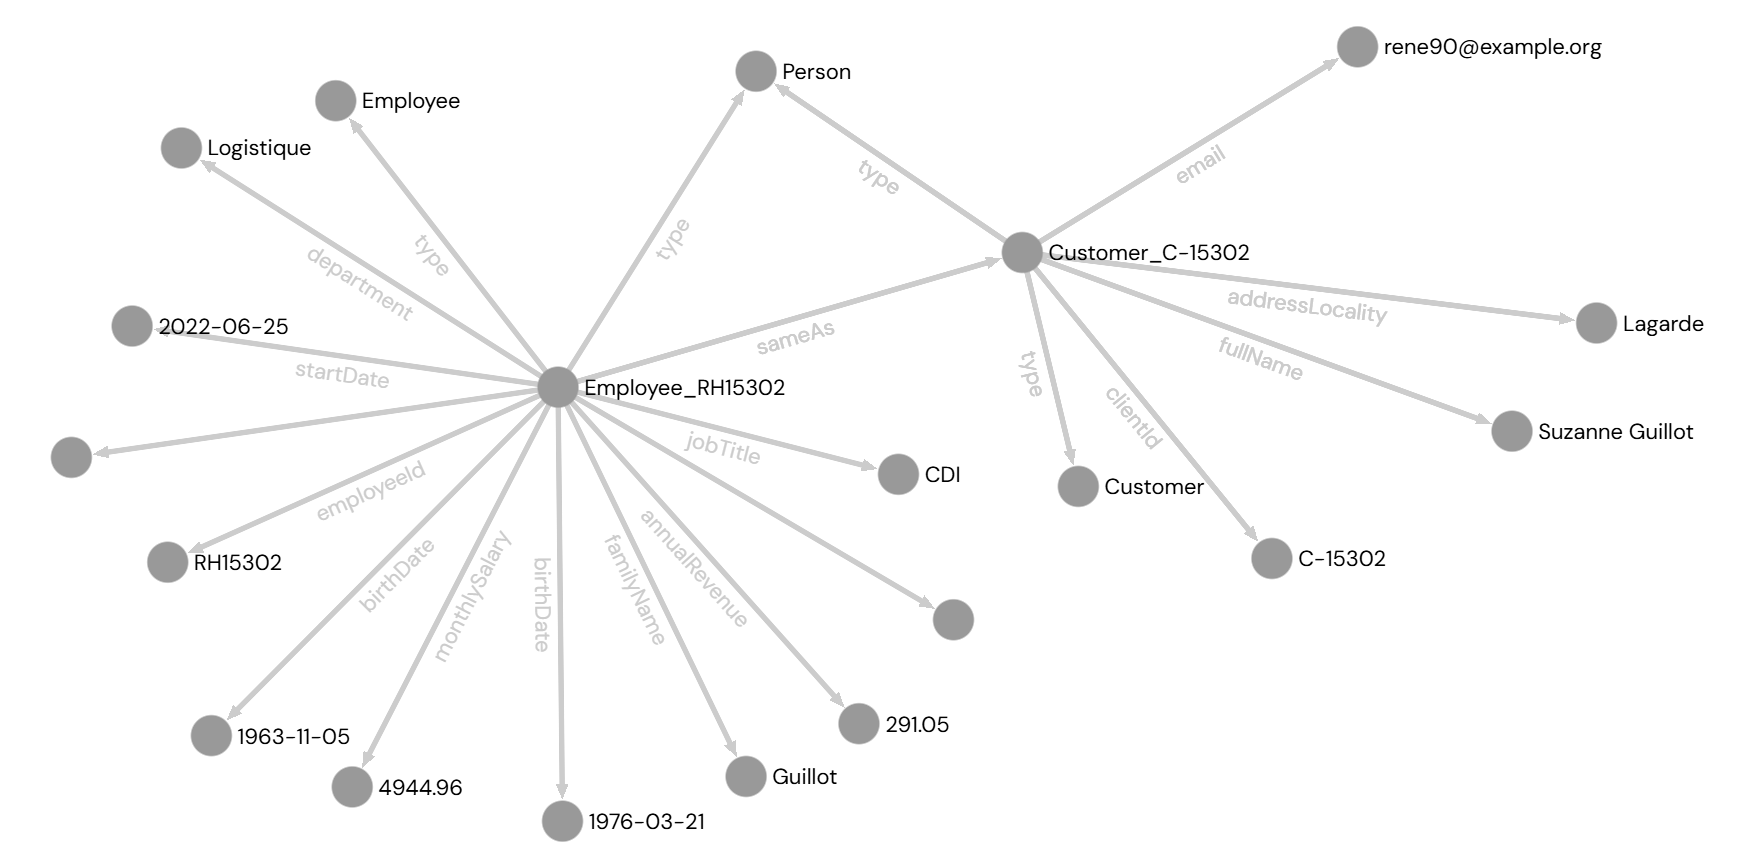
\includegraphics[width=1\textwidth]{pics/module4_splink_sameas.png}
  \caption{Illustration de la structure en «~nœud papillon~»
           (\textit{butterfly node}) produite par le Module~4~:
           un triplet \texttt{owl:sameAs} unit l'entité CRM
           (\texttt{CUST-1234}) et l'entité SIRH (\texttt{EMP-1234}).
           Les arêtes colorées représentent les triplets de propriétés
           issus de chaque source~; les arêtes rouges centrales
           matérialisent les ponts de réconciliation Splink.}
  \label{fig:module4_butterfly}
\end{figure}

%-----------------------------------------------------------------------
\section{Déploiement et Visualisation}
\label{sec:deploiement}
%-----------------------------------------------------------------------

\subsection{Stockage dans Ontotext GraphDB}
\label{subsec:graphdb}

L'ensemble des fichiers N-Triples produits (sous-graphes Source~A,
Source~B et ponts \texttt{owl:sameAs}) est chargé dans une instance
\textbf{Ontotext GraphDB~10.x}~\cite{ontotext2024graphdb}, déployée sur la
plateforme Lightning.ai. GraphDB a été retenu pour sa prise en charge
native des graphes nommés (\textit{named graphs}), sa conformité
complète au standard SPARQL~1.1, et ses performances d'inférence
OWL~2~RL qui permettent de matérialiser automatiquement les conséquences
des triplets \texttt{owl:sameAs} (propagation des propriétés d'une
entité à son équivalent sémantique).

L'upload est réalisé via l'API REST de GraphDB, paramétré pour importer
chaque fichier dans un graphe nommé distinct~:
\texttt{http://kg.projet.fr/graph/crm} pour la Source~A,
\texttt{http://kg.projet.fr/graph/sirh} pour la Source~B, et\\
\texttt{http://kg.projet.fr/graph/linkage} pour les ponts
\texttt{owl:sameAs}. Cette organisation en graphes nommés préserve
la \textbf{traçabilité de la provenance} de chaque triplet,
conformément aux recommandations de la littérature sur la gestion
de la qualité des Knowledge Graphs~\cite{hogan2021kg}.

\subsection{Visualisation interactive~: PyVis}
\label{subsec:pyvis}

Une interface de visualisation interactive du Knowledge Graph produit
a été développée à l'aide de la bibliothèque \textbf{PyVis}~\cite{pyvis2023},
qui génère un fichier HTML auto-contenu exploitable directement dans
un navigateur web, sans dépendance serveur. Cette visualisation
présente le graphe en mode \textit{force-directed} et met
particulièrement en évidence les \textbf{liens \texttt{owl:sameAs}}
produits par le Module~4~:

\begin{itemize}
  \item Les \textbf{nœuds entité} (instances de \texttt{ex:Employee}
    et \texttt{ex:Customer}) sont colorés selon leur source d'origine
    (bleu pour la Source~A, orange pour la Source~B)~;
  \item Les \textbf{arêtes de propriétés} (date de naissance, chiffre
    d'affaires, nom) relient chaque nœud à ses valeurs littérales~;
  \item Les \textbf{arêtes \texttt{owl:sameAs}} sont représentées en
    rouge, matérialisant visuellement la structure en «~nœud papillon~»
    caractéristique d'une résolution d'entités réussie.
\end{itemize}

\noindent L'interface permet de naviguer interactivement parmi les
\textbf{82\,420~triplets} stockés dans GraphDB, de filtrer par type
de relation et d'inspecter les attributs de chaque entité réconciliée.
Cette capacité d'exploration visuelle constitue un outil de validation
qualitative complémentaire aux métriques quantitatives présentées dans
les sections précédentes.

\begin{figure}[H]
  \centering
  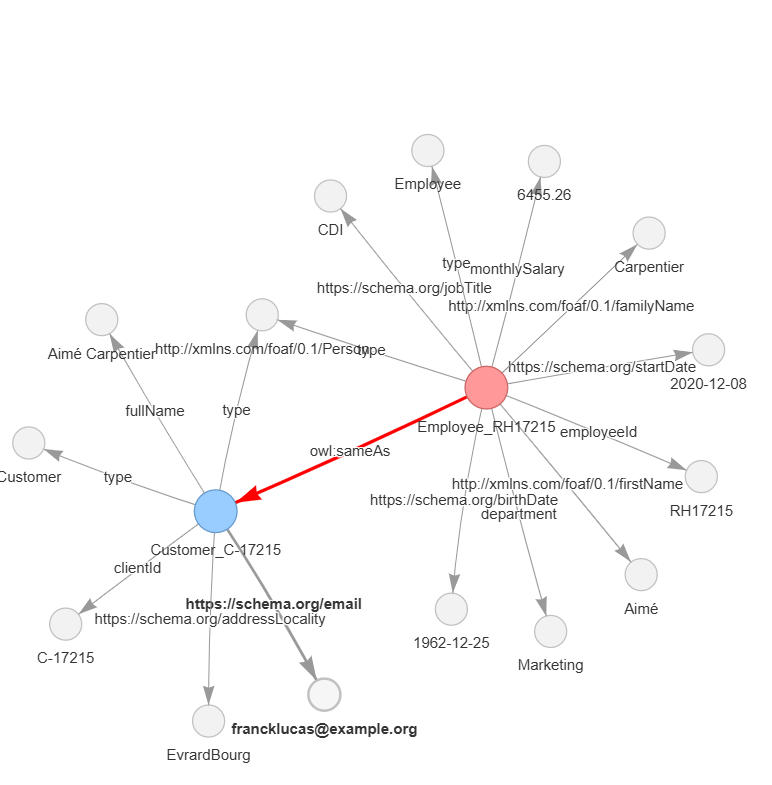
\includegraphics[width=0.8\textwidth]{pics/pyvis_kg_visualization2.png}
  \caption{Visualisation PyVis du Knowledge Graph final~: vue centrée
           sur un cluster de réconciliation. Les nœuds bleus
           (Source~A, CRM) et orange (Source~B, SIRH) sont reliés
           par des arêtes rouges \texttt{owl:sameAs} générées par
           Splink. Le fichier HTML interactif est exporté dans
           \texttt{outputs/visualization/kg\_graph.html}.}
  \label{fig:pyvis_kg}
\end{figure}

%-----------------------------------------------------------------------
\section{Bilan des Performances et Analyse Critique}
\label{sec:bilan}
%-----------------------------------------------------------------------

\subsection{Récapitulatif des temps d'exécution de bout en bout}
\label{subsec:temps_execution}

Le pipeline complet, de la génération de la vérité terrain (Module~0)
jusqu'à la sérialisation des ponts \texttt{owl:sameAs} (Module~4),
s'est exécuté en un \textbf{temps total de 46,35~secondes} sur la
plateforme Lightning.ai. Ce résultat démontre la faisabilité d'un
pipeline sémantique complet --- ingestion, profilage, schema matching
hybride, triplification, résolution d'entités --- à l'échelle de
milliers d'entités, dans un laps de temps compatible avec un usage
interactif. Le tableau~\ref{tab:bilan_temps} récapitule la
répartition du temps d'exécution par module.

\begin{table}[h]
\centering
\caption{Récapitulatif des temps d'exécution du pipeline de bout en
         bout (46,35~secondes au total).}
\label{tab:bilan_temps}
\begin{tabular}{clcc}
\hline
\textbf{Module}
  & \textbf{Intitulé}
  & \textbf{Temps (s)}
  & \textbf{Part (\%)} \\
\hline
0 & Génération et data augmentation (\texttt{Faker})          &  1,34  &  2,9  \\
1 & Ingestion et profilage (\texttt{ydata-profiling})          & 12,92  & 27,9  \\
2 & Schema matching hybride (SBERT + LLaMA~3.1/Groq)          &  6,18  & 13,3  \\
3 & Triplification sémantique (Morph-KGC)                     &  7,00  & 15,1  \\
4 & Résolution d'entités (Splink/DuckDB) + sérialisation      & 18,91  & 40,8  \\
\hline
\textbf{Total}
  &
  & \textbf{46,35}
  & \textbf{100,0} \\
\hline
\end{tabular}
\end{table}

\noindent Le Module~1 (profilage) et le Module~4 (résolution d'entités)
représentent à eux seuls \textbf{68,7\,\%} du temps total
d'exécution. Le profilage par \texttt{ydata-profiling} est
intrinsèquement coûteux car il réalise une analyse statistique
complète de chaque colonne~; cette étape pourrait être accélérée en
mode \texttt{minimal=True} déjà activé, ou désactivée en production
lorsque la qualité des sources est connue. Le Module~4 est dominé par
la phase de scoring Splink, dont la complexité est quadratique dans le
pire cas~; le backend DuckDB permet de contenir cette complexité
pour les volumes traités.

\subsection{Limites identifiées et perspectives}
\label{subsec:limites}

Plusieurs limites doivent être explicitement reconnues.

\paragraph{Données synthétiques et généralisation.}
Le pipeline a été évalué sur un jeu de données entièrement synthétique,
généré par \texttt{Faker} à partir d'un dataset transactionnel public.
Si ce choix est justifié par les impératifs de reproductibilité et de
contrôle de la vérité terrain, il limite la portée externe des
résultats~: les performances sur des données réelles, avec leurs
irrégularités, erreurs de saisie et inconsistances non contrôlées,
pourraient différer. Une validation sur un jeu de données réel
anonymisé constituerait un prolongement naturel de ce travail.

\paragraph{Sensibilité des hyperparamètres de Splink.}
Comme mis en évidence à la section~\ref{subsec:seuil_sensibilite},
le modèle Splink est fortement sensible aux paramètres de blocage.
Un blocage mal calibré peut rendre le modèle inopérant, indépendamment
du seuil de décision $\lambda$. La définition automatique de clés de
blocage adaptatives constitue une direction de recherche ouverte.

\paragraph{Dépendance à l'ontologie de domaine.}
L'architecture suppose l'existence préalable d'une ontologie OWL bien
formée. Dans les contextes où une telle ontologie n'existe pas, une
étape de construction ontologique automatique~\cite{nuzzolese2021}
serait nécessaire en amont.

\paragraph{Coût des appels LLM à très grande échelle.}
Pour des pipelines traitant des centaines de sources simultanément,
le nombre d'appels à LLaMA~3.1 via Groq~API pourrait devenir un
goulot d'étranglement en termes de latence cumulée. La substitution
par un modèle open-source déployé localement (Mistral~\cite{jiang2023mistral}
ou LLaMA via Ollama~\cite{ollama2024}) est directement supportée par
l'abstraction LangChain, sans modification de l'architecture du
Module~2.

%-----------------------------------------------------------------------
\section{Conclusion du Chapitre}
\label{sec:chap3_conclusion}
%-----------------------------------------------------------------------

Ce chapitre a présenté l'implémentation concrète et les réalisations
techniques du pipeline de transformation de données tabulaires
hétérogènes en Knowledge Graph, développé et exécuté sur la plateforme
Cloud Lightning.ai en Python~3.10.

Notre architecture s'articule autour de cinq modules séquentiels,
orchestrés par le script maître \texttt{run\_pipeline.py} et
journalisés par un \texttt{RotatingFileHandler} adapté aux contraintes
Big Data. Le \textbf{Module~0} a permis de constituer une vérité terrain
contrôlée~: 4\,000~lignes CRM (CSV) et 3\,000~lignes SIRH (Excel)
générées par \texttt{Faker} avec 1\,600~individus communs. Le
\textbf{Module~1} a attesté d'une qualité de données parfaite (0\,\% de
valeurs nulles, 0~doublon) via \texttt{ydata-profiling}. Le
\textbf{Module~2}, cœur scientifique du travail, a mis en œuvre une
architecture hybride SBERT/LLaMA~3.1 (\textit{Lazy Loading} via Groq~API),
résolvant 7~correspondances sur 8 en 6,18~secondes avec un rejet
justifié. Une \textbf{étude d'ablation comparative}
(section~\ref{sec:ablation_module2}) a confirmé empiriquement la
pertinence de ce choix architectural~: l'architecture hybride obtient
un F1-score de \textbf{0,923}, contre 0,769 pour chacune des deux
variantes isolées (SBERT seul et LLM seul), tout en étant la seule
variante capable de produire un vrai rejet correct. Le \textbf{Module~3} a généré \textbf{82\,420~triplets RDF}
via Morph-KGC et des règles YARRRML auto-générées en 7~secondes. Le
\textbf{Module~4} a illustré la sensibilité du modèle de Fellegi-Sunter
aux paramètres de blocage (0~paire candidate à $\lambda = 0{,}85$,
nécessitant un ajustement itératif), avant de produire les ponts
sémantiques \texttt{owl:sameAs} chargés dans GraphDB et visualisés
via PyVis.

Le temps total d'exécution du pipeline de bout en bout est de
\textbf{46,35~secondes}, validant la faisabilité de l'approche à
l'échelle de milliers d'entités. Ces réalisations confirment empiriquement
la pertinence des choix architecturaux défendus au
Chapitre~\ref{chap:methodologie}. Les limites identifiées --- données
synthétiques, sensibilité des hyperparamètres de blocage, dépendance
à une ontologie préexistante --- ouvrent des directions de travaux
futurs précises, discutées dans la conclusion générale du mémoire.